\documentclass[11pt, a4paper]{article}
\usepackage[a4paper, margin=2.5cm]{geometry}
\usepackage[T1]{fontenc}
\usepackage[utf8]{inputenc}
\usepackage{polski}

\usepackage{amsmath}
\usepackage{booktabs}
\usepackage{pgfplots}
\pgfplotsset{compat=1.18}
\usepackage{xcolor}
\usepackage{hyperref}

\definecolor{primary}{RGB}{30, 64, 175}
\definecolor{secondary}{RGB}{225, 29, 72}
\definecolor{tertiary}{RGB}{16, 185, 129}

\title{Algorytmy i Struktury Danych -- Laboratorium 5}
\author{Filip Będkowski}
\date{\today}

\begin{document}

\maketitle

\section{Opis zajęć}
Celem zajęć było napisanie i przeprowadzenie badań na algorytmach sortowania:
Pomiary przeprowadziłem dla tablic o rozmiarach $N \in \{100, 1000, 10000, 100000\}$ zawierających losowe elementy. Analizie poddano czas wykonania (w milisekundach), liczbę porównań oraz liczbę operacji przestawień elementów.

\section{Wyniki Pomiarów}

Poniższa tabela przedstawia szczegółowe zestawienie uzyskanych danych pomiarowych.

\begin{table}[h!]
\centering
\caption{Wyniki eksperymentu dla poszczególnych rozmiarów tablic}
\vspace{0.5em}
\begin{tabular}{c l r r r}
\toprule
\textbf{Rozmiar ($N$)} & \textbf{Algorytm} & \textbf{Czas [ms]} & \textbf{Liczba porównań} & \textbf{Przestawienia} \\
\midrule
100 & BubbleSort Opt & 0.054562 & 4 895 & 2 476 \\
    & SelectionSort & 0.029986 & 4 950 & 98 \\
    & InsertionSort & \textbf{0.022373} & \textbf{2 573} & 2 476 \\
\midrule
1 000 & BubbleSort Opt & 5.827630 & 498 680 & 247 031 \\
      & SelectionSort & 2.676080 & 499 500 & \textbf{995} \\
      & InsertionSort & \textbf{2.232020} & \textbf{248 024} & 247 031 \\
\midrule
10 000 & BubbleSort Opt & 524.253 & 49 993 824 & 25 160 550 \\
       & SelectionSort & 234.931 & 49 995 000 & \textbf{9 994} \\
       & InsertionSort & \textbf{190.547} & \textbf{25 170 541} & 25 160 550 \\
\midrule
100 000 & BubbleSort Opt & 54 795.300 & 4 999 747 434 & 2 491 127 831 \\
        & SelectionSort & 24 324.600 & 4 999 950 000 & \textbf{99 988} \\
        & InsertionSort & \textbf{19 865.800} & \textbf{2 491 227 821} & 2 491 127 831 \\
\bottomrule
\end{tabular}
\end{table}

\begin{figure}[h!]
\centering
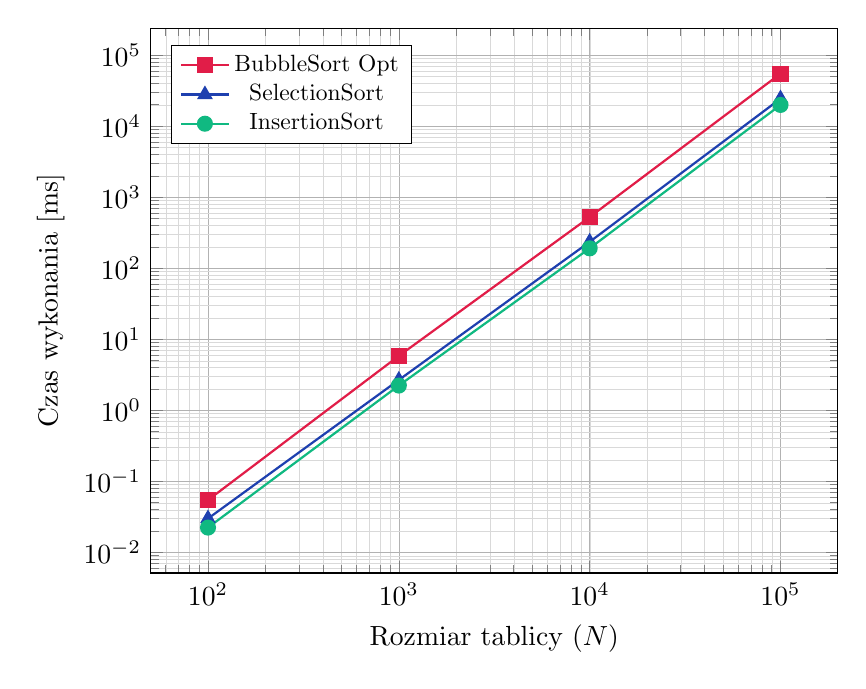
\begin{tikzpicture}
\begin{loglogaxis}[
    width=0.85\textwidth,
    height=8.5cm,
    xlabel={Rozmiar tablicy ($N$)},
    ylabel={Czas wykonania [ms]},
    grid=both,
    grid style={line width=.1pt, draw=gray!30},
    major grid style={line width=.2pt, draw=gray!60},
    legend pos=north west,
    legend style={nodes={scale=0.85, transform shape}},
    cycle list name=color list,
    mark size=2.5pt
]

\addplot[color=secondary, mark=square*, thick] coordinates {
    (100, 0.054562)
    (1000, 5.82763)
    (10000, 524.253)
    (100000, 54795.3)
};
\addlegendentry{BubbleSort Opt}

\addplot[color=primary, mark=triangle*, thick] coordinates {
    (100, 0.029986)
    (1000, 2.67608)
    (10000, 234.931)
    (100000, 24324.6)
};
\addlegendentry{SelectionSort}

\addplot[color=tertiary, mark=*, thick] coordinates {
    (100, 0.022373)
    (1000, 2.23202)
    (10000, 190.547)
    (100000, 19865.8)
};
\addlegendentry{InsertionSort}

\end{loglogaxis}
\end{tikzpicture}
\caption{Porównanie czasu wykonania algorytmów sortowania w skali log-log}
\end{figure}

\section{Analiza wyników}
InsertionSort wykazał najszybszy czas działania i najmniejszą liczbę porównań w porównaniu do BubbleSort i SelectionSort

\end{document}